% !TeX root = ../index.tex
\documentclass[../index.tex]{subfiles}
\begin{document}
    \section{Wykład 3}
        Temperaturę gwiazd można zmierzyć na kilka sposobów. Robi się to badając promieniowanie elektromagnetyczne z nich pochodzące. Pierwsze dwa sposoby korzystają z modelu ciała doskonale czarnego, natomiast trzeci z widm absorbcyjnych gwiazd:
        \begin{enumerate}
            \item \textbf{Prawo przesunięć Wiena} \--- ciało doskonale czarne  emituje najwięcej promieniowania o długości określonej przez wzór:
            \begin{equation} 
                \lambda_{\max} \cdot T = 2.898 \cdot 10^{ - 3}mK
            \end{equation} 
            \item \textbf{Prawo Stefana-Boltzmanna} \--- całkowite promieniowanie wyemitowane przez ciało doskonale czarne określa wzór:
            \begin{equation}
                F_\text{em}=\sigma \cdot T^{4}\label{eq:Stefan-Boltzmann}
            \end{equation}
            gdzie \(\sigma = 5.67 \cdot 10^{ - 8}Wm^{ - 2}K^{ - 4}\)
            \item Pierwiastki zawarte w atmosferze gwiazd pochłaniają konkretne długości fal zgodnie z prawami przejść kwantowych. Skutkiem tego jest widmo liniowe absorbcyjne \--- widmo ciągłe pozbawione niektórych częstości. Badając te częstości można dowiedzieć się jakie pierwiastki budują gwiazdę i na podstawie tego zaklasyfikować ją do konkretnego typu gwiazdowego. Gwiazdy danego typu mają podobne temperatury, więc jest to także pomiar temperatury.
        \end{enumerate}
        \subsection{Gwiazda jako ciało doskonale czarne}
            Gwiazdy są w przybliżeniu ciałami doskonale czarnymi. Jednak w widmie gwiazd można dostrzec mnóstwo linii widmowych, których nie ma w rozkładzie Plancka co wskazuje, że jest to tylko przybliżenie. W celu zrobienia użytku z formalizmu ciała doskonale czarnego wprowadzono termin \textbf{temperatury efektywnej} \--- temperatury, którą miałaby powierzchnia gwiazdy (bezpośrednio emitująca część gwiazdy \--- \textbf{fotosfera}), gdyby promieniowała jak ciało doskonale czarne.
            Gwiazdy mają różne kolory. Zgodnie z prawem przesunięć Wiena im cieplejsza gwiazd tym dla krótszej fali przypada maksimum. Zatem gwiazdy białe są cieplejsze od czerwonych, a niebieskie od białych. Mierząc długość, której przypada największe natężenie promieniowania można otrzymać temperaturę efektywną. Innym sposobem pomiaru temperatury efektywnej jest skorzystanie z prawa Stefana-Boltzmanna (\ref{eq:Stefan-Boltzmann}). Z ziemi można zmierzyć jedynie bolometryczny strumień promieniowania \(F_\text{obs}\). Wiąże się on z temperaturą efektywną wzorem:
            \begin{equation}
                4\pi R^2 \sigma T_\text{eff}^{4} = 4\pi D^2 F_\text{obs} 
            \end{equation}
            co można przekształcić do:
            \begin{equation}
                T_\text{eff}^{4} = \frac{1}{\sigma}\autoround{\frac{D}{R}}^2 F_\text{obs}
            \end{equation}
            gdzie \(D\) to odległość od gwiazdy, a \(R\) to promień gwiazdy. Niestety dla wielu gwiazd nie potrafimy dokładnie zmierzyć ich promieni ani ich odległości. Aby dokonać pomiarów temperatury takich gwiazd stosuje się \textbf{system fotometryczny Johnsona-Cousinsa}.
            \subsubsection{System fotometryczny Johnsona-Cousinsa}
                Badanie widma polega na rejestracji jasności gwiazdy za pomocą wybranych dwóch filtrów np. B i V. Różnica tych pomiarów wyrażona w skali magnitudo informuje o ilorazie strumieni promieniowania w dwóch zakresach (przepuszczanych przez filtry). Zgodnie z wzorem Pogsona:
                \begin{equation}
                    \frac{F_B}{F_V} = 10^{ - 0.4(B - V)}
                \end{equation}
                Znając ten stosunek można korzystać z tablic (stworzonych na podstawie gwiazdy, których temperatury zmierzono inaczej) wyznaczyć temperaturę gwiazdy. Metoda ta nie wymaga znajomości odległości od gwiazdy ani jej rozmiaru. Nie jest też potrzebna rejestracja widma. Niestety ze względu na obecność materii międzygwiezdnej część promieniowania nie dociera do obserwatora. To zjawisko nazywa się \textbf{ekstynkcją międzygwiazdową}. Ekstynkcja działa selektywnie \--- pochłania silniej promieniowanie o jednej częstości niż pewnej innej częstości. Głównie pochłaniane są krótsze fale \--- stąd inna nazwa efektu \--- \textbf{poczerwienienie międzygwiazdowe}.
        \subsection{Linie widmowe}
            Ekstynkcja nie likwiduje linii widmowych, więc można korzystać z ich istnienia. Każda linia widmowa jest efektem przejścia atomu z jednego stanu energetycznego do innego. Każdy pierwiastek i jego jon dysponuje pewnym unikatowym zestawem linii, które można wykorzystać do zidentyfikowania jego obecności w widmie gwiazdy. Jak za pomocą linii widmowych można uzyskać informacje na temat temperatury gwiazdy? Pierwiastki w różnych przedziałach temperatury są bardziej lub mniej zjonizowane. W pewnych przedziałach mogą nawet tworzyć związki chemiczne, a te charakteryzuję się jeszcze innymi liniami niż budujące je atomy. Przykładowo zjonizowany hel występuje w przedziale od \(10000\:K\) do \(30000\:K\). Przedział wydaje się szeroki, ale badając różne pierwiastki dostajemy więcej takich przedziałów, których przecięcia są już znacznie węższe. Temperatura ma też wpływ na to, które z możliwych linii charakterystycznych dla danego jonu mogą powstawać. Kolejne pokolenia spektroskopistów stworzyły obszerne i dokładne opisy widm różnych pierwiastków i jonów, dzięki czemu można w obserwowanym świetle doszukiwać się wystąpień poszczególnych linii widmowych.\newline
            Na podstawie występowania charakterystycznych linii w widmach
            gwiazd dokonano ich klasyfikacji, definiując tzw. \textbf{typ widmowy} gwiazdy. Oznacza się je wielkimi literami alfabetu łacińskiego. Dla większej precyzji wprowadzono pojęcie \textbf{podtypu widmowego}, oznaczanego cyfrą arabską zapisaną po literze np. B0 i B9. Aby przypisać gwiazdę do typu podtypu widmowego porównuje się jej widmo ze zestawem wzorców. Klasyfikowana gwiazda trafia do typu, którego wzorzec jej widmo przypomina najbardziej. Poniżej ukazane są najważniejsze typy widmowe uporządkowane według malejącej temperatury. Boczne gałęzie oznaczają typy widmowe wyodrębnione na podstawie nietypowej nadobfitości występowania niektórych pierwiastków.
            \begin{center}
                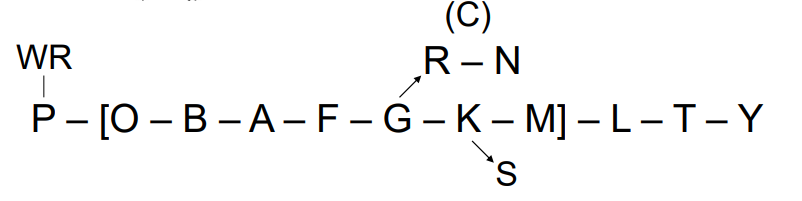
\includegraphics[width=10cm]{images/typyWidmowe.png}
            \end{center}
            Zapamiętanie 7 najważniejszych typów widmowych ułatwia wierszyk \textit{Oh Be A Fine Girl, Kiss Me!}. Typ gwiazdowy słońca to G2.
\end{document}